% !TEX program = xelatex

\RequirePackage{silence} % :-\
    \WarningFilter{scrreprt}{Usage of package `titlesec'}
    %\WarningFilter{scrreprt}{Activating an ugly workaround}
    \WarningFilter{titlesec}{Non standard sectioning command detected}
\documentclass[ twoside,openright,titlepage,numbers=noenddot,%1headlines,
                headinclude,footinclude,cleardoublepage=empty,abstract=on,
                BCOR=5mm,paper=b5,fontsize=10pt,dvipsnames
                ]{scrreprt}
\renewcommand\textsc[1]{{\fontfamily{put}\fontshape{sc}\selectfont#1}}

% use some packages
\usepackage{multicol}
\usepackage{xcolor}

%********************************************************************
% Note: Make all your adjustments in here
%*******************************************************
% !TEX program = xelatex
% ****************************************************************************************************
% classicthesis-config.tex
% formerly known as loadpackages.sty, classicthesis-ldpkg.sty, and classicthesis-preamble.sty
% Use it at the beginning of your ClassicThesis.tex, or as a LaTeX Preamble
% in your ClassicThesis.{tex,lyx} with \input{classicthesis-config}
% ****************************************************************************************************
% If you like the classicthesis, then I would appreciate a postcard.
% My address can be found in the file ClassicThesis.pdf. A collection
% of the postcards I received so far is available online at
% http://postcards.miede.de
% ****************************************************************************************************


% ****************************************************************************************************
% 0. Set the encoding of your files. UTF-8 is the only sensible encoding nowadays. If you can't read
% äöüßáéçèê∂åëæƒÏ€ then change the encoding setting in your editor, not the line below. If your editor
% does not support utf8 use another editor!
% ****************************************************************************************************
\PassOptionsToPackage{utf8}{inputenc}
  \usepackage{inputenc}

\PassOptionsToPackage{T1}{fontenc} % T2A for cyrillics
  \usepackage{fontenc}

% ****************************************************************************************************
% 1. Configure classicthesis for your needs here, e.g., remove "drafting" below
% in order to deactivate the time-stamp on the pages
% (see ClassicThesis.pdf for more information):
% ****************************************************************************************************
\usepackage[
    drafting=true,
    tocaligned=true,
    dottedtoc=true,
    eulerchapternumbers=false,
    linedheaders=false,
    palatino=true,
    beramono=true,
    floatperchapter=true,
    style=classicthesis,
    parts=true
]{classicthesis}


% ****************************************************************************************************
% 2. Personal data and user ad-hoc commands (insert your own data here)
% ****************************************************************************************************
\newcommand{\myTitle}{Animal Movement Strategies\xspace}
\newcommand{\mySubtitle}{An Homage to The Elements of Typographic Style\xspace}
\newcommand{\myDegree}{Doktor-Ingenieur (Dr.-Ing.)\xspace}
\newcommand{\myName}{Pratik Rajan Gupte\xspace}
\newcommand{\myProf}{Prof. Dr. Franz J. Weissing\xspace}
\newcommand{\myOtherProf}{Put name here\xspace}
\newcommand{\mySupervisor}{Put name here\xspace}
\newcommand{\myFaculty}{Faculty of Science and Engineering\xspace}
\newcommand{\myDepartment}{Groningen Institute for Evolutionary Life Sciences\xspace}
\newcommand{\myUni}{University of Groningen\xspace}
\newcommand{\myLocation}{Saarbrücken\xspace}
\newcommand{\myTime}{June 2018\xspace}
\newcommand{\myVersion}{\classicthesis}

% ********************************************************************
% Setup, finetuning, and useful commands
% ********************************************************************
\providecommand{\mLyX}{L\kern-.1667em\lower.25em\hbox{Y}\kern-.125emX\@}
\newcommand{\ie}{i.\,e.}
\newcommand{\Ie}{I.\,e.}
\newcommand{\eg}{e.\,g.}
\newcommand{\Eg}{E.\,g.}
% ****************************************************************************************************


% ****************************************************************************************************
% 3. Loading some handy packages
% ****************************************************************************************************
% ********************************************************************
% Packages with options that might require adjustments
% ********************************************************************
\PassOptionsToPackage{ngerman,american}{babel} % change this to your language(s), main language last
% Spanish languages need extra options in order to work with this template
%\PassOptionsToPackage{spanish,es-lcroman}{babel}
    \usepackage{babel}

\usepackage{csquotes}
\PassOptionsToPackage{%
  backend=biber,
  hyperref,
  url=false,
  isbn=false,
  doi=false,
  eprint=false,
  style=oxyear,%oxyear, % Author 1999, 2010
  dashed=true, % dashed: substitute rep. author with ---
  maxcitenames=2,
  maxbibnames=99, % default: 3, et al.
  date=year,
  uniquename=false,
  uniquelist=false,
  useprefix=true,
  sortcites=true,
  sorting=ynt, % name, year, title
  % sortfirstinits=true, % for handling names with prefixes, e.g. le Roux to be with Romano, not Leclerc.
  natbib=true % natbib compatibility mode (\citep and \citet still work)
}{biblatex}
\usepackage{biblatex}

% REMOVE THE MONTH WHICH LEADS TO EMPTY () AFTER THE ENTRY
% \AtEveryBibitem{\clearfield{pages}}
% \AtEveryBibitem{\clearfield{volume}}
\AtEveryBibitem{\clearfield{month}}
\AtEveryCitekey{\clearfield{month}}

% try to remove empty brackets
% \renewbibmacro*{issue+date}{%
%   \ifboolexpr{test {\iffieldundef{issue}} and test {\iffieldundef{year}}}
%     {}
%     {\printtext[parens]{%
%        \printfield{issue}%
%        \setunit*{\addspace}%
%        \usebibmacro{date}}%
%      \newunit}}

% % more code to remove empty brackets
% \renewbibmacro*{url+urldate}{%
%   \iffieldundef{url}
%     {}
%     {\printtext[parens]{%
%        \printfield{url}
%        \setunit{\addsemicolon\space}%
%        \printurldate}}}

\PassOptionsToPackage{fleqn}{amsmath}       % math environments and more by the AMS
  \usepackage{amsmath}

% ********************************************************************
% General useful packages
% ********************************************************************
\usepackage{graphicx} %
\usepackage{scrhack} % fix warnings when using KOMA with listings package
\usepackage{xspace} % to get the spacing after macros right
\PassOptionsToPackage{printonlyused,smaller}{acronym}
  \usepackage{acronym} % nice macros for handling all acronyms in the thesis
  %\renewcommand{\bflabel}[1]{{#1}\hfill} % fix the list of acronyms --> no longer working
  %\renewcommand*{\acsfont}[1]{\textsc{#1}}
  %\renewcommand*{\aclabelfont}[1]{\acsfont{#1}}
  %\def\bflabel#1{{#1\hfill}}
  \def\bflabel#1{{\acsfont{#1}\hfill}}
  \def\aclabelfont#1{\acsfont{#1}}
% ****************************************************************************************************
%\usepackage{pgfplots} % External TikZ/PGF support (thanks to Andreas Nautsch)
%\usetikzlibrary{external}
%\tikzexternalize[mode=list and make, prefix=ext-tikz/]
% ****************************************************************************************************


% ****************************************************************************************************
% 4. Setup floats: tables, (sub)figures, and captions
% ****************************************************************************************************
\usepackage{tabularx} % better tables
  \setlength{\extrarowheight}{3pt} % increase table row height
\newcommand{\tableheadline}[1]{\multicolumn{1}{l}{\spacedlowsmallcaps{#1}}}
\newcommand{\myfloatalign}{\centering} % to be used with each float for alignment
\usepackage{subfig}
% ****************************************************************************************************


% ****************************************************************************************************
% 5. Setup code listings
% ****************************************************************************************************
\usepackage{listings}
%\lstset{emph={trueIndex,root},emphstyle=\color{BlueViolet}}%\underbar} % for special keywords
\lstset{language=[LaTeX]Tex,%C++,
  morekeywords={PassOptionsToPackage,selectlanguage},
  keywordstyle=\color{RoyalBlue},%\bfseries,
  basicstyle=\small\ttfamily,
  %identifierstyle=\color{NavyBlue},
  commentstyle=\color{Green}\ttfamily,
  stringstyle=\rmfamily,
  numbers=none,%left,%
  numberstyle=\scriptsize,%\tiny
  stepnumber=5,
  numbersep=8pt,
  showstringspaces=false,
  breaklines=true,
  %frameround=ftff,
  %frame=single,
  belowcaptionskip=.75\baselineskip
  %frame=L
}

\lstdefinestyle{customR}{
  belowcaptionskip=1\baselineskip,
  captionpos=b,
  breaklines=true,
%   numbers=left,
  frame=L,
  xleftmargin=\parindent,
  language=R,
  showstringspaces=false,
  basicstyle=\small\ttfamily\color{black},
  keywordstyle=\ttfamily,
  commentstyle=\color{commentstyleCol},   % comment style
  stringstyle=\color{stringstyleCol}      % string literal style
}
% ****************************************************************************************************




% ****************************************************************************************************
% 6. Last calls before the bar closes
% ****************************************************************************************************
% ********************************************************************
% Her Majesty herself
% ********************************************************************
\usepackage{classicthesis}

% ********************************************************************
% Fine-tune hyperreferences (hyperref should be called last)
% ********************************************************************
\hypersetup{%
  %draft, % hyperref's draft mode, for printing see below
  colorlinks=true, linktocpage=true, pdfstartpage=3, pdfstartview=FitV,%
  % uncomment the following line if you want to have black links (e.g., for printing)
  %colorlinks=false, linktocpage=false, pdfstartpage=3, pdfstartview=FitV, pdfborder={0 0 0},%
  breaklinks=true, pageanchor=true,%
  pdfpagemode=UseNone, %
  % pdfpagemode=UseOutlines,%
  plainpages=false, bookmarksnumbered, bookmarksopen=true, bookmarksopenlevel=1,%
  hypertexnames=true, pdfhighlight=/O,%nesting=true,%frenchlinks,%
  urlcolor=CTurl, 
  linkcolor=, 
  citecolor=black, %pagecolor=RoyalBlue,%
  %urlcolor=Black, linkcolor=Black, citecolor=Black, %pagecolor=Black,%
  pdftitle={\myTitle},%
  pdfauthor={\textcopyright\ \myName, \myUni, \myFaculty},%
  pdfsubject={},%
  pdfkeywords={},%
  pdfcreator={pdfLaTeX},%
  pdfproducer={LaTeX with hyperref and classicthesis}%
}


% ********************************************************************
% Setup autoreferences (hyperref and babel)
% ********************************************************************
% There are some issues regarding autorefnames
% http://www.tex.ac.uk/cgi-bin/texfaq2html?label=latexwords
% you have to redefine the macros for the
% language you use, e.g., american, ngerman
% (as chosen when loading babel/AtBeginDocument)
% ********************************************************************
\makeatletter
\@ifpackageloaded{babel}%
  {%
    \addto\extrasamerican{%
      \renewcommand*{\figureautorefname}{Figure}%
      \renewcommand*{\tableautorefname}{Table}%
      \renewcommand*{\partautorefname}{Part}%
      \renewcommand*{\chapterautorefname}{Chapter}%
      \renewcommand*{\sectionautorefname}{Section}%
      \renewcommand*{\subsectionautorefname}{Section}%
      \renewcommand*{\subsubsectionautorefname}{Section}%
    }%
    \addto\extrasngerman{%
      \renewcommand*{\paragraphautorefname}{Absatz}%
      \renewcommand*{\subparagraphautorefname}{Unterabsatz}%
      \renewcommand*{\footnoteautorefname}{Fu\"snote}%
      \renewcommand*{\FancyVerbLineautorefname}{Zeile}%
      \renewcommand*{\theoremautorefname}{Theorem}%
      \renewcommand*{\appendixautorefname}{Anhang}%
      \renewcommand*{\equationautorefname}{Gleichung}%
      \renewcommand*{\itemautorefname}{Punkt}%
    }%
      % Fix to getting autorefs for subfigures right (thanks to Belinda Vogt for changing the definition)
      \providecommand{\subfigureautorefname}{\figureautorefname}%
    }{\relax}
\makeatother


% ********************************************************************
% Development Stuff
% ********************************************************************
\listfiles
%\PassOptionsToPackage{l2tabu,orthodox,abort}{nag}
%  \usepackage{nag}
%\PassOptionsToPackage{warning, all}{onlyamsmath}
%  \usepackage{onlyamsmath}


% ****************************************************************************************************
% 7. Further adjustments (experimental)
% ****************************************************************************************************

%\DeclareRobustCommand{\spacedallcaps}[1]{\color{Black} \textls[90]{\bfseries\scshape\large{\MakeTextUppercase{#1}}} \par}

%\DeclareRobustCommand{\maintitle}[1]{{\fontsize{70}{50}\selectfont {\scshape{#1}}\par}}
      
%\DeclareRobustCommand{\spacedlowsmallcaps}[1]{\textls[80]{{#1}}}

%\DeclareRobustCommand{\tocchapter}[1]{{{#1}}}
%\DeclareRobustCommand{\tocpart}[1]{{\bfseries\large{#1}}}

% ********************************************************************
% Changing the text area
% ********************************************************************
%\areaset[current]{312pt}{761pt} % 686 (factor 2.2) + 33 head + 42 head \the\footskip
%\setlength{\marginparwidth}{7em}%
%\setlength{\marginparsep}{2em}%

% ********************************************************************
% Using different fonts
% ********************************************************************
%\usepackage[oldstylenums]{kpfonts} % oldstyle notextcomp
%\usepackage[osf]{libertine}
%\usepackage{libertine}
%\usepackage{fonts}
%\usepackage[T1]{fontenc}
%\usepackage[usefilenames,RMstyle=Light,SSstyle=Light,TTstyle=Light,DefaultFeatures={Ligatures=Common}]{plex-otf}
%\usepackage[light,condensed,math]{iwona}
%\renewcommand{\sfdefault}{iwona}
%\usepackage{lmodern} % <-- no osf support :-(
%\usepackage{cfr-lm} %
%\usepackage[urw-garamond]{mathdesign} <-- no osf support :-(
%\usepackage[default,osfigures]{opensans} % scale=0.95
%\usepackage[sfdefault]{FiraSans}
% \usepackage[opticals,mathlf]{MinionPro} % onlytext
% ********************************************************************
%\usepackage[largesc,osf]{newpxtext}
%\linespread{1.05} % a bit more for Palatino
% Used to fix these:
% https://bitbucket.org/amiede/classicthesis/issues/139/italics-in-pallatino-capitals-chapter
% https://bitbucket.org/amiede/classicthesis/issues/45/problema-testatine-su-classicthesis-style
% ********************************************************************
% ****************************************************************************************************


%********************************************************************
% Bibliographies
%*******************************************************
% \RequirePackage[authoryear,sort]{natbib}

\addbibresource{chapters/preprocessing.bib}
% \addbibresource{Bibliography.bib}
% \addbibresource[label=ownpubs]{AMiede_Publications.bib}

%********************************************************************
% Hyphenation
%*******************************************************
%\hyphenation{put special hyphenation here}

\usepackage{sourcesanspro}   % scaling is recommended
\setmainfont[Ligatures=TeX]{Source Serif Pro}
\setsansfont{Source Sans Pro}

\newfontfamily\myfont{TeX Gyre Pagella}
\newfontfamily\numfont{TeX Gyre Schola}

\renewcommand{\chapterNumber}{%
  \color{Black}\fontsize{60}{60} \bfseries\numfont}\par

\makeatletter
% fix part heading format
\titleformat{\part}[display]
        {\ct@altfont\centering\LARGE\rmfamily}%
        {\thispagestyle{empty}\scshape\myfont\partname~\MakeTextUppercase{\thepart}}{1em}%
        {\color{Maroon}\scshape\bfseries\huge\myfont}[\bigskip\normalfont\normalsize\color{Black}\begin{quote}\ctparttext@print\end{quote}]
        
% fix chapter heading format
\titleformat{\chapter}[display]%
    % \setbox0=\hbox{\chapterNumber\thechapter\hspace{10pt}\vline\ }%
    {\relax}{\mbox{}\oldmarginpar{\chapterNumber\thechapter}}{0pt}%
    {\raggedright\huge\emph}[\normalsize\vspace*{.8\baselineskip}\titlerule]%

% fix section format
\titleformat{\section}
    {\relax}{\textsc{\MakeTextLowercase{\thesection}}}{1em}{\bfseries\scshape\large\color{Maroon}\myfont}

% parts in toc
\renewcommand{\cftpartfont}{\color{Maroon}\scshape\bfseries}%
% chapters in toc
\renewcommand{\cftchappresnum}{\normalfont}%
\renewcommand{\cftchapaftersnumb}{\normalfont}%
\renewcommand{\cftchapfont}{\normalfont}%
\renewcommand{\cftchappagefont}{\normalfont}%
\makeatother

% ********************************************************************
% GO!GO!GO! MOVE IT!
%*******************************************************
\begin{document}
\frenchspacing
\raggedbottom
\selectlanguage{american} % american ngerman
%\renewcommand*{\bibname}{new name}
%\setbibpreamble{}
% \pagenumbering{roman}
\pagestyle{plain}
%********************************************************************
% Frontmatter
%*******************************************************
% %*******************************************************
% Little Dirty Titlepage
%*******************************************************
\thispagestyle{empty}
%\pdfbookmark[1]{Titel}{title}
%*******************************************************
\begin{center}
    \spacedlowsmallcaps{\myName} \\ \medskip

    \begingroup
        \color{CTtitle}\spacedallcaps{\myTitle}
    \endgroup
\end{center}

%*******************************************************
% Cover Titlepage
%*******************************************************
\definecolor{myOrange}{rgb}{0.969,0.965,0.945}

\begin{titlepage}
    \pagecolor{myOrange}\afterpage{\nopagecolor}
    %\pdfbookmark[1]{\myTitle}{titlepage}
    % if you want the titlepage to be centered, uncomment and fine-tune the line below (KOMA classes environment)
    \begin{addmargin}[-1cm]{-3cm}
    % \begin{center}
        \linespread{1.5}
        % \large

        \hfill

        % \vfill
        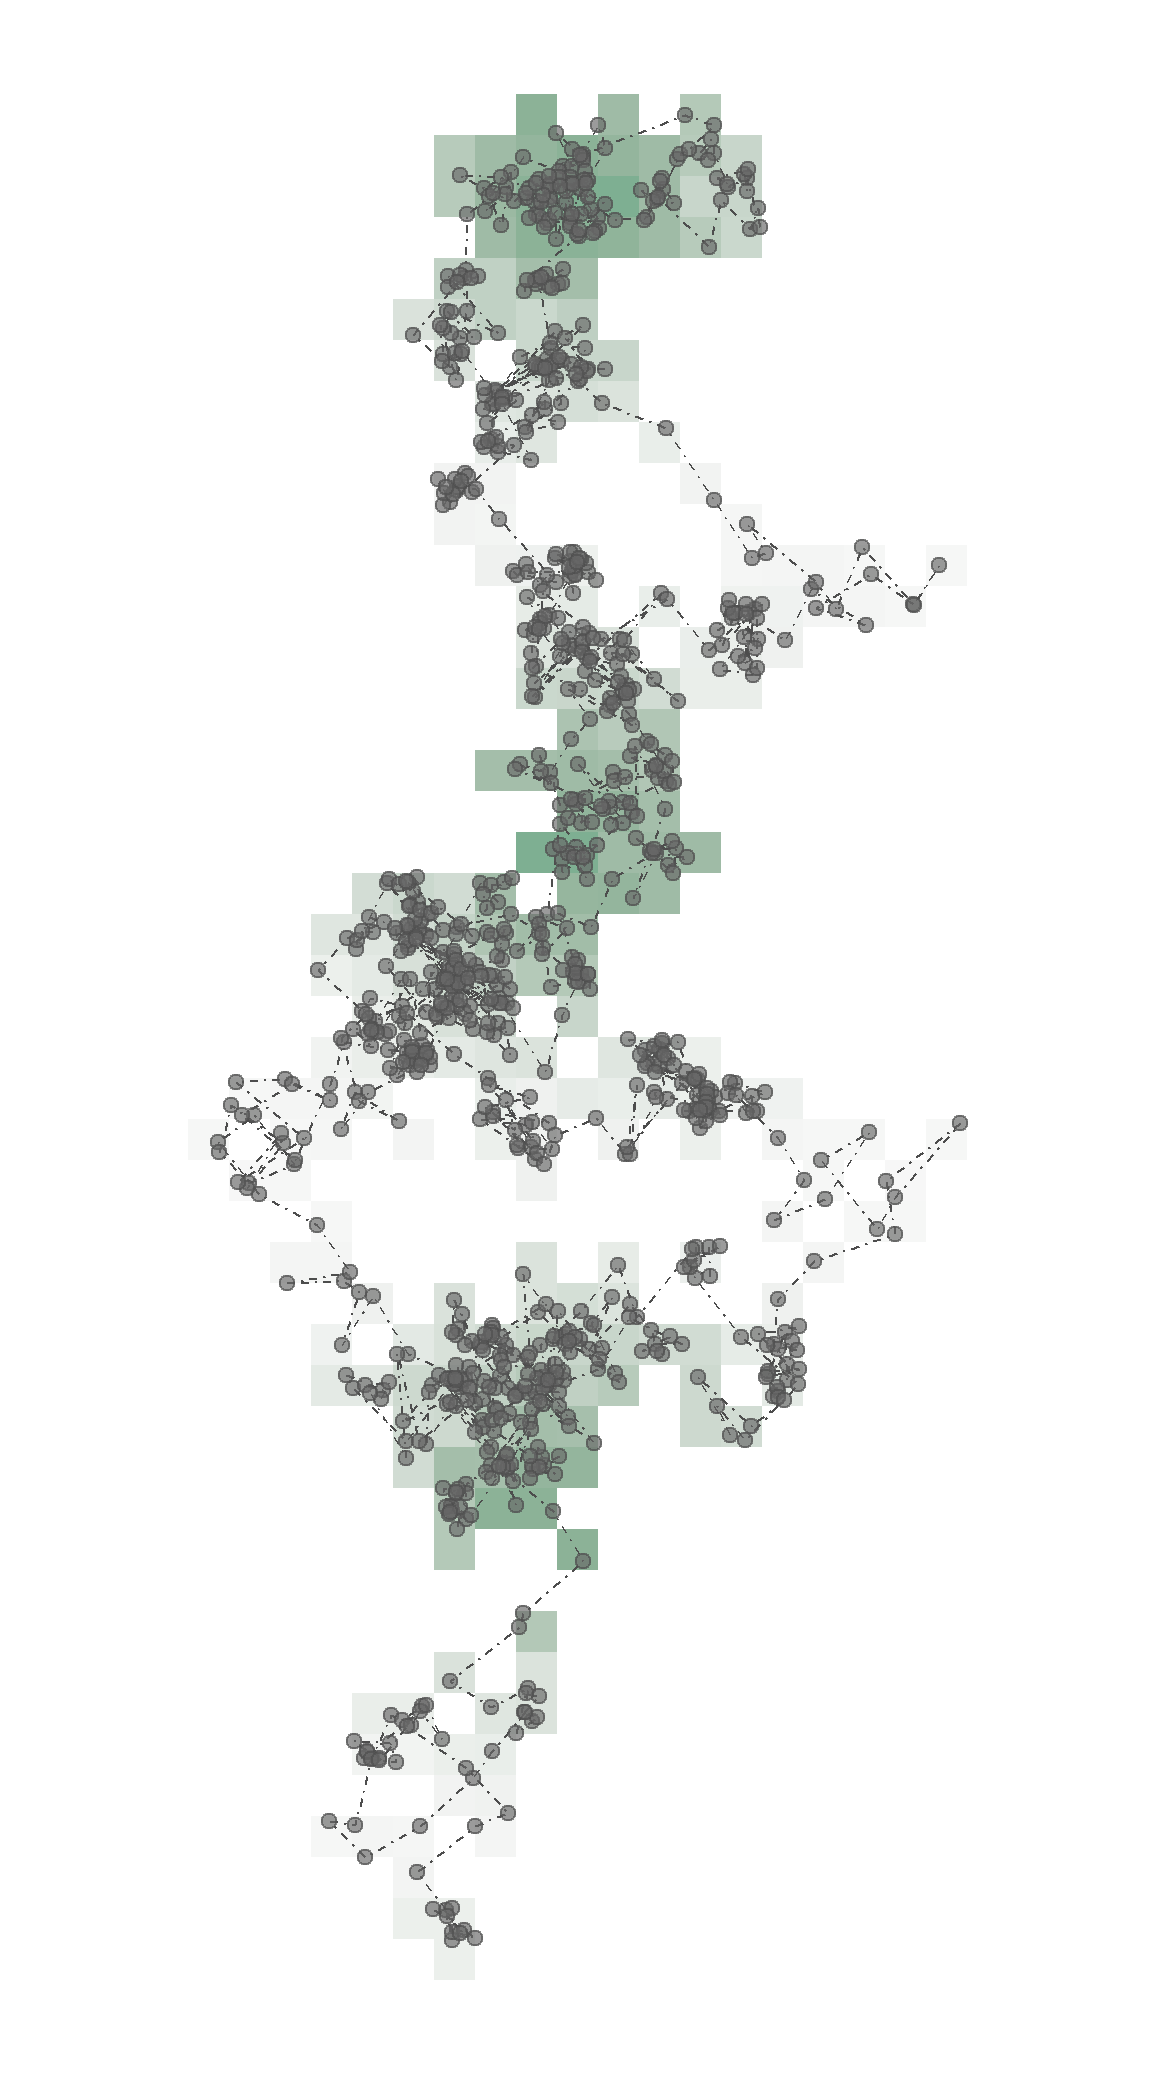
\includegraphics[width=1.0\textwidth,
          align=h,
          smash=br,
          hsmash=r,
          hshift=0.5\textwidth,
          % vshift=1cm,     % adjust the vertical position
          % hshift=-1.5cm
          ]{figures/cover_2.png}
        {
          \begin{flushleft}
            \color{SteelBlue4}{\fontsize{60}{50} \bfseries\sffamily{ANIMAL\\MOVEMENT\\STRATEGIES}\par}\par
          \end{flushleft}
        }
        % \makebox[0pt][h]{%
          % \raisebox{-\totalheight}[0pt][0pt]{%
        
          % }
        % }%
        \vspace{81mm}

        \sffamily\huge{PRATIK RAJAN GUPTE}

        \vfill

        % \includegraphics[width=6cm]{gfx/TFZsuperellipse_bw} \\ \medskip

        % \mySubtitle \\ \medskip
        %\myDegree \\
        %\myDepartment \\
        %\myFaculty \\
        %\myUni \\ \bigskip

        % \myTime\ -- \myVersion

        \vfill

    % \end{center}
  \end{addmargin}
\end{titlepage}

\nopagecolor

\thispagestyle{empty}

\hfill

\vfill

\noindent {\scshape{COLOPHON}}

\noindent The research presented in this thesis was carried out at the Department for Theoretical Research in Evolutionary Life Sciences (TRES), at the Groningen Institute for Evolutionary Life Sciences (GELIFES), at the University of Groningen's Faculty of Science and Engineering (FSE).
This research was made possible by an \emph{Adaptive Life} grant from GELIFES; part of the work in this thesis was funded by the European Research Council (ERC Advanced Grant No. 789240).
Support for this research was provided primarily by the University of Groningen; other institutions whose support made parts of this work possible are acknowledged within.
The production of this thesis was partly funded by GELIFES, the FSE, and the University of Groningen.

\medskip

\noindent This document was typeset using the \emph{classicthesis} \LaTeX~style, developed by Andr\'e Miede and Ivo Pletikosić.
% This style was inspired by Robert Bringhurst's seminal book on typography \emph{The Elements of Typographic Style}.
The text is mostly set in \emph{Timepos Text} from the New Zealand-based Klim Type Foundry, with some headings in \emph{Plex Serif} from the Dutch type foundry Bold Monday. Friedrich Althausen's \emph{Vollkorn} is used for chapter breaks.

\bigskip

\noindent\finalVersionString

\noindent\myName. \textit{\myTitle.}% \mySubtitle, %\myDegree,
\\
\noindent \textcopyright\ \today

% \cleardoublepage%*******************************************************
% Dedication
%*******************************************************
\thispagestyle{empty}
\phantomsection
\pdfbookmark[1]{Dedication}{Dedication}

\vspace*{3cm}

\begin{center}
    \large\emph{What can be achieved by not listening to supervisors}
    
\end{center}
%\cleardoublepage\include{FrontBackmatter/Foreword}
% \cleardoublepage\pagestyle{empty}

\hfill

\vfill


\pdfbookmark[0]{Colophon}{colophon}
\section*{Colophon}
This document was typeset based on \emph{classicthesis}, developed by Andr\'e Miede and Ivo Pletikosić.
The style was inspired by Robert Bringhurst's seminal book on typography ``\emph{The Elements of Typographic Style}''.
Inspired by Wouter Vahl's PhD thesis ``\emph{Interference Competition in Foraging Waders}'', Matthew Carter's Charter is used for the main text; Vernon Adams' Oswald is used for headings.
The cover design is inspired by the colours of the Japanese edition of Theodore M. Porter's ``\emph{Trust the Numbers}''.

\bigskip

\noindent\finalVersionString

%Hermann Zapf's \emph{Palatino} and \emph{Euler} type faces (Type~1 PostScript fonts \emph{URW
%Palladio L} and \emph{FPL}) are used. The ``typewriter'' text is typeset in \emph{Bera Mono},
%originally developed by Bitstream, Inc. as ``Bitstream Vera''. (Type~1 PostScript fonts were made
%available by Malte Rosenau and
%Ulrich Dirr.)

%\paragraph{note:} The custom size of the textblock was calculated
%using the directions given by Mr. Bringhurst (pages 26--29 and
%175/176). 10~pt Palatino needs  133.21~pt for the string
%``abcdefghijklmnopqrstuvwxyz''. This yields a good line length between
%24--26~pc (288--312~pt). Using a ``\emph{double square textblock}''
%with a 1:2 ratio this results in a textblock of 312:624~pt (which
%includes the headline in this design). A good alternative would be the
%``\emph{golden section textblock}'' with a ratio of 1:1.62, here
%312:505.44~pt. For comparison, \texttt{DIV9} of the \texttt{typearea}
%package results in a line length of 389~pt (32.4~pc), which is by far
%too long. However, this information will only be of interest for
%hardcore pseudo-typographers like me.%
%
%To make your own calculations, use the following commands and look up
%the corresponding lengths in the book:
%\begin{verbatim}
%    \settowidth{\abcd}{abcdefghijklmnopqrstuvwxyz}
%    \the\abcd\ % prints the value of the length
%\end{verbatim}
%Please see the file \texttt{classicthesis.sty} for some precalculated
%values for Palatino and Minion.
%
%    \settowidth{\abcd}{abcdefghijklmnopqrstuvwxyz}
%    \the\abcd\ % prints the value of the length

\cleardoublepage
\cleardoublepage% Table of Contents
%*******************************************************
\begingroup
\raggedright
% \pagestyle{scrheadings}
\thispagestyle{empty}
\phantomsection
\pdfbookmark[1]{\contentsname}{tableofcontents}
\setcounter{tocdepth}{0} % <-- 2 includes up to subsections in the ToC
\setcounter{secnumdepth}{2} % <-- 3 numbers up to subsubsections
\manualmark
\markboth{\spacedlowsmallcaps{\contentsname}}{\spacedlowsmallcaps{\contentsname}}
\begin{onehalfspace}

    \raggedright
    \tableofcontents

    \automark[section]{chapter}
    % \renewcommand{\chaptermark}[1]{\markboth{\spacedlowsmallcaps{#1}}{\spacedlowsmallcaps{#1}}}
    % \renewcommand{\sectionmark}[1]{\markright{\textsc{\thesection}\enspace\spacedlowsmallcaps{#1}}}
\end{onehalfspace}

\endgroup
\cleardoublepage

\cleardoublepage%*******************************************************
% Abstract
%*******************************************************
%\renewcommand{\abstractname}{Abstract}
\pdfbookmark[1]{Abstract}{Abstract}
% \addcontentsline{toc}{chapter}{\tocEntry{Abstract}}
\begingroup
% \let\clearpage\relax
% \let\cleardoublepage\relax
% \let\cleardoublepage\relax

\chapter*{Abstract}

% \begin{center}
%     \emph{What are birds, if not dinosaurs persevering?}\\
%     \medskip
%     -- \small{Paraphrased from \textit{WandaVision}, 2021.}
% \end{center}

% Competition typically takes place in a spatial context, but eco-evolutionary models rarely address the joint evolution of movement and competition strategies. 
% Here we investigate a spatially explicit forager-kleptoparasite model where consumers can either forage on a heterogeneous resource landscape, or steal resource items from conspecifics (kleptoparasitism). 
% We consider three scenarios: (1) foragers without kleptoparasites; (2) consumers specializing as foragers or as kleptoparasites; and (3) consumers that can switch between foraging and kleptoparasitism depending on local conditions.
% We model movement strategies as individual-specific combinations of preferences for environmental cues, similar to step-selection coefficients.
% By means of mechanistic, individual-based simulations, we study the joint evolution of movement and competition strategies, and we investigate the implications on the resource landscape and the distribution of consumers over this landscape.
% Movement and competition strategies evolve rapidly and consistently across all scenarios, with marked differences among scenarios, leading to differences in resource exploitation patterns.
% % The evolved movement and resource exploitation patterns differ considerably across the three scenarios.
% In scenario 1, foragers evolve considerable individual variation in movement strategies, while in scenario 2, movement strategy is tightly correlated with competition strategy, with a swift divergence between foragers and kleptoparasites.
% When individuals' competition strategy is conditional on local cues, movement strategies converge to facilitate kleptoparasitism, and individual consistency in competition strategy also emerges.
% Across scenarios, the distribution of consumers over resources differs substantially from `ideal free' predictions. 
% This is related to the intrinsic difficulty of moving effectively on a depleted resource landscape with few reliable cues for movement.
% Our study emphasises the advantages of a mechanistic approach when studying competition in a spatial context, and suggests how evolutionary modelling can be integrated with current work in animal movement ecology.

% \begin{center}
% % \url{https://plg.uwaterloo.ca/~migod/research/beckOOPSLA.html}
% \end{center}

% \vfill

% \begin{otherlanguage}{ngerman}
% \pdfbookmark[1]{Zusammenfassung}{Zusammenfassung}
% \chapter*{Zusammenfassung}
% Kurze Zusammenfassung des Inhaltes in deutscher Sprache\dots
% \end{otherlanguage}

\endgroup

\vfill

\clearpage

%********************************************************************
% Mainmatter
%*******************************************************
% \cleardoublepage
\pagestyle{scrheadings}
\pagenumbering{arabic}
%\setcounter{page}{90}
% use \cleardoublepage here to avoid problems with pdfbookmark
% \cleardoublepage


\phantomsection
\addtocontents{toc}{\protect\vspace{\beforebibskip}}%
% \addcontentsline{toc}{chapter}{\tocEntry{\color{black}\itshape{General Introduction: The Current Frontiers of Animal Movement Ecology}}}%
\chapter{General Introduction: The Current Frontiers of Animal Movement Ecology}\label{ch:introduction}
\chaptermark{General Introduction}

{{Pratik R. Gupte}}

% \begin{center}
%     \emph{Coming back to where you started is not the same as never leaving.}\\
%     \medskip
%     -- \small{Terry Pratchett}
% \end{center}

% Movement is a fascinating phenomenon.
% It integrates a deep, implicit \textit{feel} for the fundamental organisation of the universe, with surprising agency: that things, colloquially speaking, need not be the same, or different.
% All animals move, whether actively or passively, at some stage of their lives.
% As humans, we have projected our own motivations on to animals around us, and arrived at a relatively good understanding of why animals move, i.e., the ecological drivers of animal movement.
% In this, we have the advantage of not being too far from our own past, before we had quite successfully insulated ourselves from the effects of such drivers.
% This allows us to take the perspective of other animals when looking at a landscape; essentially, to mentally \textit{model} movement decisions across it.

% {\color{red} WORK IN PROGRESS}

To be completed.

\vfill

\clearpage


% Competition typically takes place in a spatial context, but eco-evolutionary models rarely address the joint evolution of movement and competition strategies. 
% Here we investigate a spatially explicit forager-kleptoparasite model where consumers can either forage on a heterogeneous resource landscape, or steal resource items from conspecifics (kleptoparasitism). 
% We consider three scenarios: (1) foragers without kleptoparasites; (2) consumers specializing as foragers or as kleptoparasites; and (3) consumers that can switch between foraging and kleptoparasitism depending on local conditions.
% We model movement strategies as individual-specific combinations of preferences for environmental cues, similar to step-selection coefficients.
% By means of mechanistic, individual-based simulations, we study the joint evolution of movement and competition strategies, and we investigate the implications on the resource landscape and the distribution of consumers over this landscape.
% Movement and competition strategies evolve rapidly and consistently across all scenarios, with marked differences among scenarios, leading to differences in resource exploitation patterns.

% \label{ch:intro}
% \addcontentsline{toc}{chapter}{\nameref{ch:intro}}

\ctparttext{You can put some informational part preamble text here.
Illo principalmente su nos. Non message \emph{occidental} angloromanic
da. Debitas effortio simplificate sia se, auxiliar summarios da que,
se avantiate publicationes via. Pan in terra summarios, capital
interlingua se que. Al via multo esser specimen, campo responder que
da. Le usate medical addresses pro, europa origine sanctificate nos se.}

\part{Tracking Animal Movement at High Resolution}

%************************************************
\chapter{High-throughput Tracking in Animal Movement Ecology}\label{ch:htme}
\chaptermark{High-throughput Animal Tracking}
%************************************************

{\noindent \sffamily Ran Nathan, \ldots \textbf{Pratik R. Gupte} \ldots and Ivan Jaric}

\section*{Abstract}

\graffito{
    \bigskip

    {\large{$\Delta$}} Published in \textit{Science} as Nathan et al.
}

\noindent Abstract redacted until publication of Nathan et al.

\clearpage


% \cleardoublepage

%************************************************
\chapter{Pre-processing High Throughput Animal Tracking Data}\label{ch:preprocessing}
%************************************************
% 
\noindent \textbf{Pratik R. Gupte}, Christine E. Beardsworth\textsuperscript{1}, Orr Spiegel\textsuperscript{2}, Emmanuel Lourie\textsuperscript{3}, Sivan Toledo\textsuperscript{2}, Ran Nathan\textsuperscript{3}, and Allert Bijleveld\textsuperscript{1}

\marginpar{
    \textsuperscript{1} Netherlands Inst. for Sea Research, The Netherlands.
    
    \medskip
    
    \textsuperscript{2} Tel Aviv University, Israel.
    
    \medskip

    \textsuperscript{3} The Hebrew University of Jerusalem, Israel.
}

\section*{Abstract}

\footnotesize{
    Modern, high-throughput animal tracking increasingly yields `big data' at very fine temporal scales. 
    At these scales, location error can exceed the animal's step size, leading to mis-estimation of behaviours inferred from movement. 
    `Cleaning' the data to reduce location errors is one of the main ways to deal with position uncertainty. 
    Though data cleaning is widely recommended, inclusive, uniform guidance on this crucial step, and on how to organise the cleaning of massive datasets, is relatively scarce.
    A pipeline for cleaning massive high-throughput datasets must balance ease of use and computationally efficiency, in which location errors are rejected while preserving valid animal movements. 
    Another useful feature of a pre-processing pipeline is efficiently segmenting and clustering location data for statistical methods, while also being scalable to large datasets and robust to imperfect sampling. 
    Manual methods being prohibitively time consuming, and to boost reproducibility, pre-processing pipelines must be automated.
    We provide guidance on building pipelines for pre-processing high-throughput animal tracking data to prepare it for subsequent analyses. 
    We apply our proposed pipeline to simulated movement data with location errors, and also show how large volumes of cleaned data can be transformed into biologically meaningful `residence patches', for exploratory inference on animal space use. 
    We use tracking data from the Wadden Sea ATLAS system (WATLAS) to show how pre-processing improves its quality, and to verify the usefulness of the residence patch method. 
    Finally, with tracks from Egyptian fruit bats \textit{Rousettus aegyptiacus}, we demonstrate the pre-processing pipeline and residence patch method in a fully worked out example.
    To help with fast implementation of standardised methods, we developed the R package \textit{atlastools}, which we also introduce here. 
    Our pre-processing pipeline and \textit{atlastools} can be used with any high-throughput animal movement data in which the high data-volume combined with knowledge of the tracked individuals’ movement capacity can be used to reduce location errors. 
    \textit{atlastools} is easy to use for beginners, while providing a template for further development. 
    The common use of simple yet robust pre-processing steps promotes standardised methods in the field of movement ecology and leads to better inferences from data.

    \medskip

    \noindent {\large{\color{Maroon}$\Delta$}} Published in the \textit{Journal of Animal Ecology} as Gupte et al. (2021). A guide to pre-processing high throughput tracking data.
}

\clearpage

% \begin{refsection}
%     \section{Introduction}

%     The movement of an animal is an adaptive, integrated response to multiple drivers, including internal state, life-history traits and capacities, biotic interactions, and other environmental factors \cite{nathan2008a, holyoak2008}.
%     % Movement has both beneficial and detrimental consequences for individual fitness, and 
%     The movement ecology framework links the drivers, processes, and fitness outcomes of animal movement \cite{nathan2008a}, and remotely tracking individual animals in the wild is the methodological mainstay of movement ecology \cite{wikelski2007,nathan2008a,hussey2015,kays2015}.
%     A key challenge with observed tracks is to extract information on the behavioural, cognitive, social, ecological and evolutionary processes that shape animal movement.
%     Addressing this challenge requires investigating the relationships between movement and its drivers at the fine scales at which animals sense and respond to variation in their environment. 
%     Tracking data, which are observations of a continuous process (animal movement) at discrete timesteps, reveal useful information about the movement process when the tracking interval is considerably shorter than the typical duration of a movement mode \cite{nathan2008a, noonan2019, getz2008}.
%     This can be accomplished by wildlife tracking systems that collect position data from many individuals at high temporal and spatial resolution (i.e., high-throughput tracking) relative to the scale of the movement mode of interest \cite{getz2008}.
%     High-throughput tracking technologies include GPS tags \cite{strandburg-peshkin2015, papageorgiou2019, harel2016, klarevas-irby2021}, tracking radars \cite{horvitz2014}, and computer vision methods for tracking entire groups of animals from video recordings \cite{rathore2020, perez-escudero2014}. 
%     Furthermore, high-throughput wildlife tracking is routinely provided by terrestrial reverse-GPS systems such as ATLAS \cite[Advanced Tracking and Localization of Animals in real-life Systems:][]{toledo2014, weiser2016, toledo2016,toledo2020} --- see also \cite{maccurdy2009, maccurdy2019} --- and underwater acoustic reverse-GPS tracking of aquatic animals \cite{baktoft2019, baktoft2017, jung2015, aspillaga2021, aspillaga2021a}.
%     Finally, low resolution tracking over a long duration may also capture important aspects of animal behaviour at certain time-scales \cite[e.g. migration, long-range dispersal;][]{getz2008}, thereby being `relatively' high-throughput.

%     Although high-throughput tracking provides a massive amount of data on the path of a tracked animal, these data present a challenge to ecologists.
%     When tracking animals at a high temporal resolution, the location error of each position may approach or exceed the true movement distance of the animal, compared to low-resolution tracking with the same measurement error.
%     This leads to an over-estimation of the true distance moved by an animal between two discrete time-points, leading to unreliable behavioural metrics ultimately derived from movement distance, such as speed and tortuosity \cite[see][]{ranacher2016, noonan2019, hurford2009, calenge2009}.
%     Additionally, the location error around a position introduces uncertainty when studying the relationship between animal movements and either fixed landscape features (e.g. roads), or mobile elements (e.g. other tracked individuals), as well as confounding estimates of habitat selection.
%     Users have two main options to improve data quality, \textit{(i)} making inferences after modelling the system-specific location error using a continuous time movement model \cite{fleming2014a, fleming2020, jonsen2003, jonsen2005, johnson2008, patterson2008, aspillaga2021}, or \textit{(ii)} pre-processing data to clean it of positions with large location errors \cite{bjorneraas2010}.
%     The first approach may be limited by the animal movement models that can be fitted to the data \cite{fleming2014a, noonan2019, fleming2020}, may result in unreasonable computation times, or may be entirely beyond the computational capacity of common hardware, leading users to prefer data cleaning instead.
%     Data cleaning reveals another challenge of high-throughput tracking: the large number of observations make it difficult for researchers to visually examine each animal's track for errors \cite{weiser2016, toledo2020}.
%     With manual identification and removal of errors from individual tracks prohibitively time consuming, data cleaning can benefit from automation based on a protocol.

%     Pre-processing of movement data --- defined as the set of data management steps executed prior to data analysis --- must reliably discard large location errors, also called outliers, from tracks (analogous to reducing false positives) while avoiding the overzealous rejection of valid animal movements (analogous to reducing false negatives).
%     How well researchers balance these imperatives has consequences for downstream analyses \cite{stine2001}.
%     For instance, small-scale resource selection functions can easily infer spurious preference and avoidance effects when there is uncertainty about an animal's true position \cite{visscher2006}.
%     Ecologists recognise that tracking data are imperfect observations of the underlying movement process, yet they implicitly consider cleaned data equivalent to the ground-truth.
%     This assumption is reflected in popular statistical methods in movement ecology such as Hidden Markov Models (HMMs) \cite{langrock2012}, stationary-phase identification methods \cite{patin2020a}, or step-selection functions (SSFs) \cite{barnett2008, signer2017, avgar2016}, which expect minimal location errors relative to real animal movement (i.e., a high signal-to-noise ratio).
%     This makes the reproducible, standardised removal of location errors crucial to any animal tracking study.
%     While gross errors are often removed by positioning-system algorithms in both GPS and reverse-GPS setups, `reasonable’ errors often remain to confront end users \cite{fischler1981, weiser2016, ranacher2016}.
%     Further, as high-throughput tracking is deployed in more regions and for more species, standardised pre-processing steps should be general enough to tackle animal movement data recovered from a range of environments, so as to enable sound comparisons across species and ecosystems.

%     Despite the importance and ubiquity of reducing location errors in tracking data, movement ecologists lack formal guidance on this crucial step.
%     Pre-processing protocols are not often reported in the literature, or may not be easily tractable for mainstream computing hardware and software.
%     Some tracking data, such as GPS, are autonomously pre-processed without user access to the raw data \cite[using error estimates and Kalman smooths;][and substantial location errors may yet persist]{kaplan2005}.
%     However, filtering out positions using estimates of location error alone may not be sufficient to exclude outliers which represent unrealistic movement but have low error measures \cite{weiser2016, ranacher2016}.
%     When tracking systems do make their raw data available to researchers, this can enable users to better control the data pre-processing stage, and to substantially improve data quality while ensuring that cleaning does not itself lead to unrealistic movement tracks \cite[e.g. Kalman smooths which distort tracks,][]{kaplan2005}.
%     Furthermore, 
%     This makes identifying and removing biologically implausible locations from a track an important component of recovering true animal movement \cite{bjorneraas2010}.
%     Even after removing unrealistic movement, a track may be comprised of positions that are randomly distributed around the true animal location \cite{noonan2019}.
%     The large data-volumes of high-throughput tracking allow for a neat solution: tracks can be `median smoothed' to reduce small location errors that have remained undetected \cite[e.g.][]{bijleveld2016} 
%     Large data volumes may also need to be thinned, for example, examining environmental covariates as predictors of prolonged residence in an area  \cite[see e.g.][]{bracis2018, aarts2008, bijleveld2016, oudman2018, harel2016} might require thinning of high-resolution movement data to match the lower spatial resolution of environmental measurements. 
%     Data thinning and clustering are also required to avoid non-independent observations due to strong spatio-temporal autocorrelation, or to examine the effect of sampling scale on movement metrics and resource-selection \cite{fleming2014a,noonan2019}.

%     When dealing with datasets that contain many millions of positions, reseachers may run into computational limits when trying to apply pre-processing steps to their full dataset.
%     For instance, the size of working memory (RAM) limits the size of datasets that can be loaded into \textit{R}, the programming and statistical language of choice in movement ecology \cite{r2020,joo2020,joo2020b}.
%     Data-rich fields such as genomics inspire a possible solution: to break very large data into smaller subsets, and pass these subsets through automated computational `pipelines' \cite{schadt2010,peng2011}.
%     Pre-processing pipelines for animal tracking data --- the set of steps that users apply to prepare the data for a specific analysis --- come with some additional concerns: \textit{(i)} identifying which pre-processing steps are necessary, and \textit{(ii)} ensuring that these steps reproducibly operate on the data as expected, and as efficiently as possible.
%     While exploratory data analysis and visualisation can help determine how to pre-process the data to maximise the signal to noise ratio \cite{slingsby2016}, standardising implementations of pre-processing techniques into robust, version controlled software packages \cite[e.g. in \textit{R}, see]{wickham2015}, can increase the reliability and reproducibility of animal movement ecology \cite{haddaway2015,archmiller2020,powers2019,lewis2018}.
%     Overcoming hard computational constraints on speed and memory usage for very large data will often require a combination of programming strategies, such as using tools optimised for tabular data, or parallelised processing.

%     Here, we present guidelines for reproducibly pre-processing high-throughput animal tracking data (Fig. 1), with a focus on simple, widely generalisable steps that help improve data quality (Fig. 2).
%     We take two important considerations into account, that \textit{(i)} the pre-processing steps should be easily understood and reproduced, and \textit{(ii)} our implementations must be computationally efficient and reliable.
%     Consequently, formalising tools as functions in an \textit{R} package would improve portability and reproducibility \cite{marwick2018, wickham2015}.
%     Using simulated movement tracks, we demonstrate simple yet robust implementations of the pre-processing steps we recommend, conveniently wrapped into the \textit{R} package \textit{atlastools} \cite{gupte2020a}, with a discussion of features that make these steps more reproducible, and more efficient.
%     We also suggest one potential application of high-throughput tracking in studies of animal movement and space use, illustrated by the first-principles based synthesis of `residence patches' from clusters of spatio-temporally proximate positions \cite[\textit{sensu}][]{bijleveld2016, oudman2018, barraquand2008}.
%     In two fully worked out examples using our package on real tracking data, we show how to apply basic spatio-temporal and data quality filters, how to filter out unrealistic movement, and how to reduce the effect of location error with a median smooth.
%     In the first example, using calibration data from an ATLAS system, we show how the residence patch segmentation-clustering method can be used to accurately identify areas of prolonged residence under real field conditions.
%     Finally, in our second example, we use ATLAS data from Egyptian fruit bats (\textit{Rousettus aegyptiacus}) tracked in the Hula Valley, Israel, to show a fully worked out example of the pre-processing pipeline and the residence patch method.
%     While our approach to high-throughput tracking data, and our package of pre-processing functions was developed with reverse-GPS ATLAS systems in mind, both are broadly suitable to a wide range of high-throughput animal tracking data sources, from underwater acoustic reverse-GPS \cite{baktoft2019, baktoft2017, jung2015, aspillaga2021, aspillaga2021a}, high-resolution GPS \cite{strandburg-peshkin2015, papageorgiou2019, harel2016, klarevas-irby2021}, tracking radars \cite{horvitz2014}, and visual video tracking \cite{rathore2020, perez-escudero2014}.

%     \section{Best-Practices for Pre-Processing Workflows}

%     % \begin{figure}
%     %     \centering
%     %     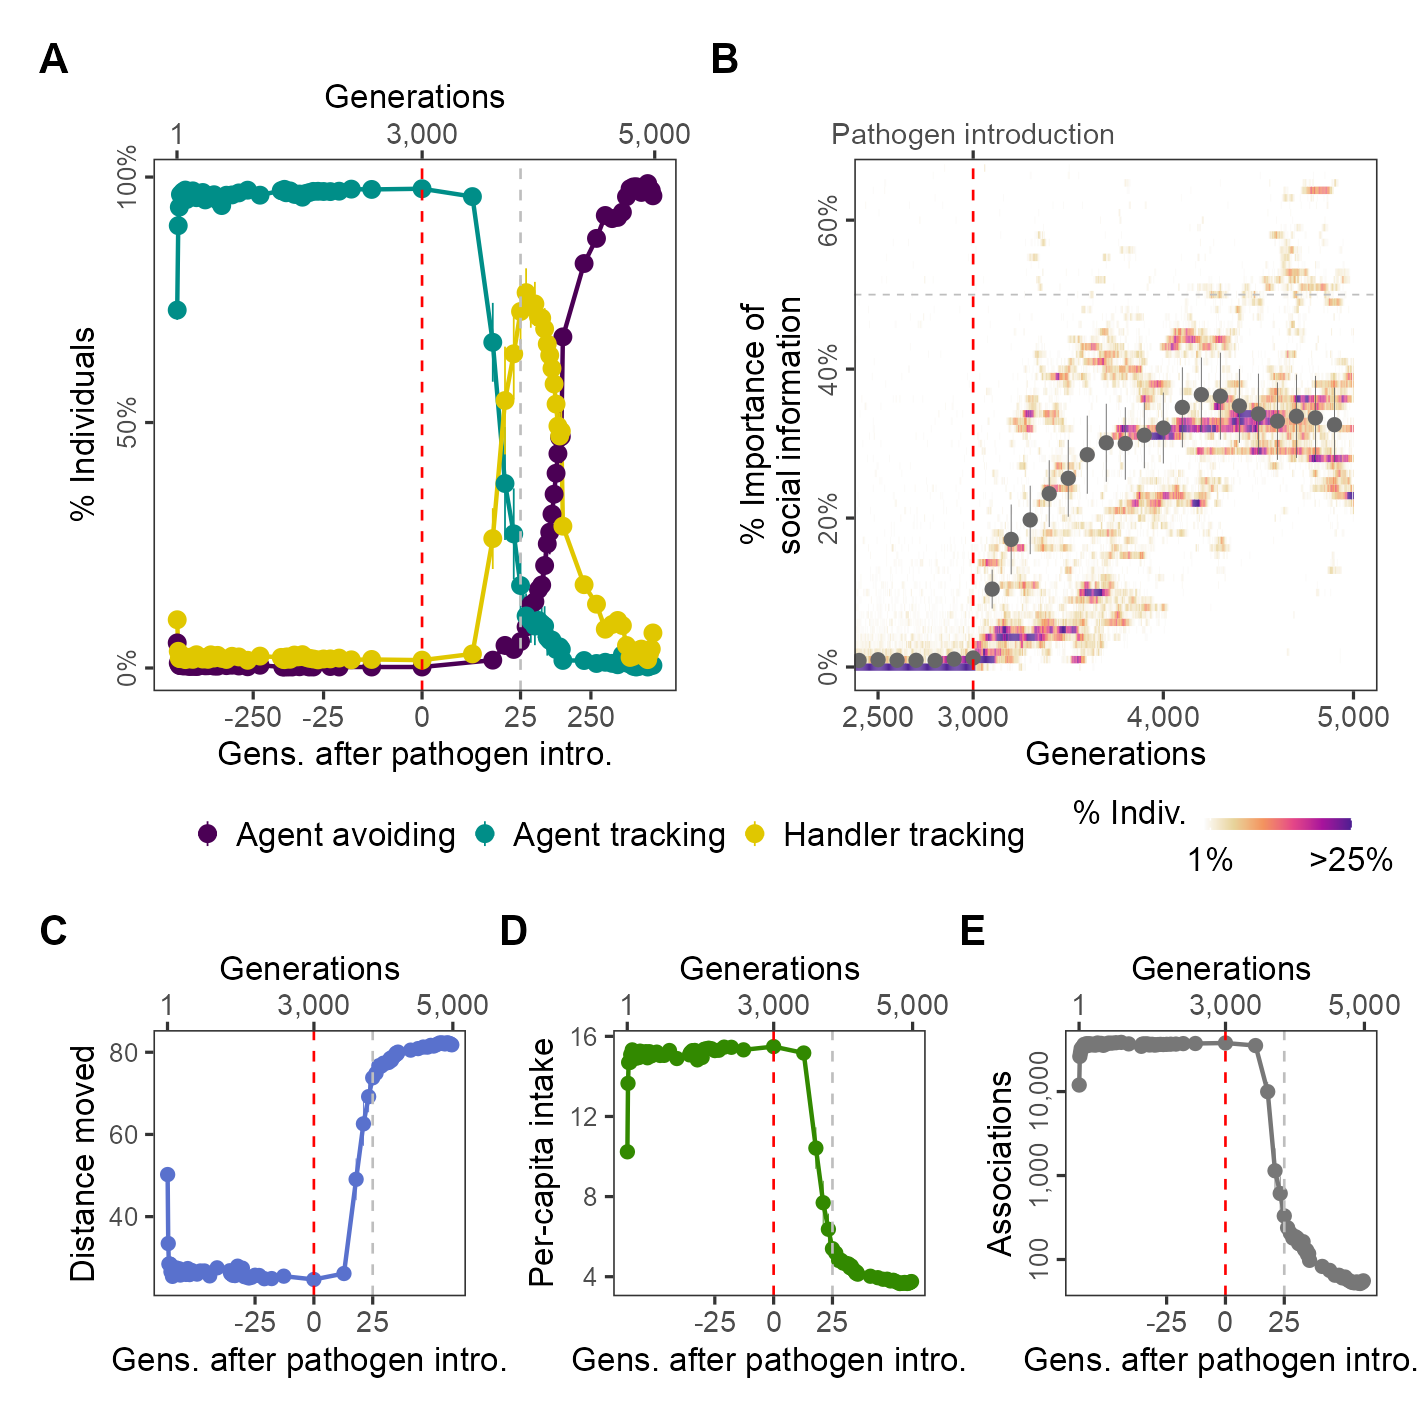
\includegraphics[width=0.95\textwidth]{figures/fig_01.png}
%     %     \caption{
%     %         \textbf{Some best-practices for pre-processing high-throughput tracking data.}\\
%     %         Simple pre-processing of animal tracking data can improve the quality of animal tracking data, and the inferences that are drawn from it.
%     %         The organisation of pre-processing workflows into a `pipeline' --- a set of steps that users apply to prepare the data for a specific analysis --- can help make research more reproducible and reliable.
%     %         Exploratory data analysis of representative subsets of the data can help to identify common issues with data quality, and to determine which pre-processing, steps such as filters and smooths, might be necessary (\textit{see also Fig. 2}).
%     %         Pre-processing steps implemented as programming code can be made reproducible and shareable by following best-practices for software development: (1) tracking changes to the steps, and the software used, using version control (e.g. \textit{git}, \textit{renv}), (2) preferring pre-existing tools, such as \textit{R} packages, which are well documented and tested, (3) encapsulating custom-written code as functions, and bundling related functions into a package, and (4) checking the quality of both custom-written code (e.g. by testing functions), and the overall pipeline (e.g. data visualisation).
%     %         The efficiency of pre-processing steps can be increased by using strategies for dealing with large datasets, such as batch processing, or using a computing cluster.
%     %         The use of existing tools optimised for large datasets, or by writing code in a `fast' language such as \textit{C++}, can also speed up the pre-processing of large datasets (see main text for examples).
%     %         See the \textsc{Worked Out Example} on Egyptian fruit bats, as well as Supplementary Material 1, for more details on implementing pipelines.
%     %         Fig. 2 shows an example of such a pipeline.
%     %     }
%     %     \label{fig:figure_concept}
%     % \end{figure}

%     \subsection{Exploratory Data Analysis to Identify Pre-processing Steps}

%     Exploratory data analysis should be the first step towards pre-processing movement data \cite[see Fig. 1;][]{slingsby2016}.
%     Researchers with very large datasets of perhaps millions of rows should ideally select a representative subset of these data for exploratory data analysis, including individuals of different species, sexes, or seasonal cohorts.
%     Examples of exploratory data analysis include plotting heatmaps of the number of observations per unit area across the study site (Fig. 1).
%     Histograms of the location error estimates, plotting the linear approximations of animal paths between observations, and histograms of the sampling interval can help determine how data need to be treated so as to minimise location errors and improve computational tractability (Fig. 1).
%     While pre-processing steps required for datasets will differ between studies and tracking technologies, we elaborate upon candidate steps and their parameterisation in following sections (see also Fig. 2).

%     \subsection{Improving Reliability and Reproducibility}

%     Following exploratory data analysis and the parameterisation of data cleaning steps, the specific implementation of these steps should be made reliable and reproducible.
%     Since reproducing pre-processing steps can be challenging when using only written descriptions from published articles, providing the code to implement pre-processing steps reduces ambiguity and increases reproducibility \cite{haddaway2015}.
%     For technically advanced users, the best-practices here are \textit{(1)} to implement pre-processing steps as `functions', \textit{(2)} to collect related functions --- e.g. for similar kinds of data --- into a software `package', \textit{(3)} to `test' that the functions handle input as expected, and \textit{(4)} implement `version control' throughout, such that the process of development is documented \cite[Fig. 1;][]{wickham2015,alston2020,perez-riverol2016}.
%     As an example, our \textit{atlastools} package incorporates these best-practices, and may be used as a reference \cite[][]{gupte2020a}.
%     We have written each pre-processing step as a separate function, and each of these functions is tested, usually on simulated data, but in some cases also on empirical data \cite[][see the directory \textit{tests/} in the associated Zenodo repository]{wickham2015}.
%     % The tests include `use cases', i.e., ensuring the functions perform calculations correctly, but also `abuse cases', which check that the functions handle unexpected inputs usefully, such as by printing informative error messages.
%     Finally, logging error messages is crucial when passing data through a pipeline, helping determine which data subsets could not be handled as expected, and why.
%     Users who would prefer to rely on pre-existing toolsets and methods can use \textit{R} packages that follow these best-practices, such as \textit{move} \cite{kranstauber2011}, and \textit{sftrack} \cite{boone2020}.

%     \subsection{Improving Speed and Efficiency}

%     The large size of modern, high-throughput animal tracking data means that the computational challenge can often be \textit{the} main challenge in working with these data.
%     For beginning users, organising their workflows so that they process subsets of the data (such as one individual) at a time can help overcome limitations on working memory.
%     Animal tracking data stored in a relational database \cite[e.g. SQL databases][]{codd1970}, for example, can be broken into meaningful subsets based on individual identity and tracking season.
%     These smaller subsets can then be loaded into working memory, pre-processed, and saved in a separate location (see Supplementary Material 1, Section 2 for a worked out example on an SQL database).
%     Using existing tools optimised for tabular data, such as the \textit{R} package \textit{data.table} \cite{dowle2020}, can also speed up computation; \textit{atlastools} is built using \textit{data.table} for this reason.
%     More advanced users seeking substantial speed gains might wish to look into parallel-processing, and process each subset of the data independently of the full dataset, for example by using a computing cluster \cite[see also][for an alternative]{zjdai2021}.
%     Finally, another advanced method, used by popular packages such as \textit{move} \cite{kranstauber2011} and \textit{recurse} \cite{bracis2018}, is to write one's own methods in a `fast' low-level language, such as \textit{C++}, and link these to \textit{R} \cite[][]{eddelbuettel2013}; see also \textit{adehabitatLT}, which is written partially in \textit{C}: \cite{calenge2006}.
%     Beginning practitioners can organise their workflows around these packages to benefit from the features they incorporate.

%     \printbibliography[heading=subbibliography]
% \end{refsection}


% \ctparttext{You can put some informational part preamble text here.
% Illo principalmente su nos. Non message \emph{occidental} angloromanic
% da. Debitas effortio simplificate sia se, auxiliar summarios da que,
% se avantiate publicationes via. Pan in terra summarios, capital
% interlingua se que. Al via multo esser specimen, campo responder que
% da. Le usate medical addresses pro, europa origine sanctificate nos se.}

% \cleardoublepage

\part{Ecology of Animal Movement and Space Use}

%************************************************
\chapter{Individual Consistency in Movement Tendencies Across Spatial Scales}\label{ch:knots}
\chaptermark{Personality \& Movement}
%************************************************

{\noindent \sffamily Selin Ersoy, \textbf{Pratik R. Gupte}, Christine E. Beardsworth, and Allert I. Bijleveld}

\section*{Abstract}

% \graffito{
%     \bigskip

%     {\large{$\Delta$}} Under review at The American Naturalist as Gupte et al. The joint evolution of animal movement and competition strategies.
% }
\small{
    Foraging is essential for many species and understanding factors affect foraging decision is a core topic in ecology.
    Patch-use theory examines how animals make decisions on when to approach and leave a particular foraging patch.
    Even though the individual factors associated with patch movement such as searching and processing the food item or digestive costs were studied under this theory, consistent individual differences (also knows as personalities) were understudied.
    Here we investigated if exploratory personality measured in controlled settings predicts patch movement in the field on red knots.
    We first assayed exploratory tendency of red knots in controlled settings (notably without food) and then release the same birds with transmitters to investigate foraging patch movements in the field.
    We asked how exploration speed in the controlled settings relates to within and between patch movement of an individual during low tide.
    We found that faster exploring red knots visit more patches during low tide and they move faster and stay shorter within the patch.
    The size of the foraging patch did not differ between individuals with different exploratory scores.
    Our findings suggest that exploration measured in captivity predicts exploration in the field, and further provides a framework to study and understand how personality variation may be maintained in populations.

    \noindent {\color{red} WORK IN PROGRESS}
}

\clearpage


% \cleardoublepage

%************************************************
\chapter{Direct Effects of Wing Moult on the Movement and Habitat Selection of Sub-tropical Birds}\label{ch:holeybirds}
\chaptermark{Wing Moult \& Movement}
%************************************************

{\noindent \sffamily\textbf{Pratik R. Gupte}, Yosef Kiat\textsuperscript{1}, Sivan Toledo\textsuperscript{2}, and Ran Nathan\textsuperscript{3}}

\marginpar{
    \sffamily
    \textsuperscript{1} University of Haifa, Israel.
    
    \medskip
    
    \textsuperscript{2} Tel Aviv University, Israel.
    
    \medskip

    \textsuperscript{3} The Hebrew University of Jerusalem, Israel.
}

\section*{Abstract}

% \marginpar{ 
%     \bigskip

%     {\large{\color{Maroon}$\Delta$}} \normalfont Published in the \textit{Journal of Animal Ecology} as Gupte et al. (2021). A guide to pre-processing high throughput tracking data.
% }

\small{
    The feathered flight of birds requires regular renewal of the wing surface through moult, the process of shedding worn out feathers and growing fresh ones.
    Moult presents birds with the dilemma of needing to move more to acquire resources for feather growth, at precisely the time that their flight capacity is reduced (due to missing wing feathers) and they are vulnerable to predation.
    Despite this central importance of moult to avian ecology, and especially to movement, we know little about its direct effects on the spatial ecology of birds.
    We combined a range of mechanistic approaches to present a first quantification of the direct, short-term effects of wing moult on the movement and habitat selection of four different non-migratory, sub-tropical birds.
    We quantified landscape visibility from a predator viewpoint, and followed the movement of birds in different stages of moult, with a high-throughput position tracking system.
    We found that birds balanced the needs and risks of moult by adjusting their movement to their wing condition.
    Naturally moulting birds moved more than non-moulting birds, but birds with wing feathers experimentally removed moved less.
    Among similarly vegetated areas, birds preferred low-visibility sheltered sites in our agricultural landscape, regardless of their moult status.
    Intriguingly, our results suggest that birds' cognitive abilities may extend to seeing a landscape from the spatial perspective of another individual.   
}

\clearpage



% \cleardoublepage

%************************************************
\chapter{Land-cover and Climate Shape Bird Occupancy in a Tropical Biodiversity Hotspot}\label{ch:hillybirds}
\chaptermark{Citizen Science \& Bird Distributions}
%************************************************
% Using citizen science to parse climatic and land cover influences on

{\noindent \sffamily Vijay Ramesh\textsuperscript{1}, \textbf{Pratik R. Gupte}, Morgan Tingley\textsuperscript{2}, V.V. Robin\textsuperscript{3}, and Ruth S. de Fries\textsuperscript{1}}

\marginpar{
    \sffamily
    \textsuperscript{1} Columbia University, USA.
    
    \medskip
    
    \textsuperscript{2} University of California --- Los Angeles, USA.
    
    \medskip

    \textsuperscript{3} Indian Institute for Science Education and Research --- Tirupati, India.
}

\section*{Abstract}

\marginpar{ 
    \bigskip

    {\large{\color{Maroon}$\Delta$}} \normalfont Under review at \textit{Ecography} as Ramesh et al. Using citizen science to parse climatic and land cover influences on bird occupancy within a tropical biodiversity hotspot.
}

\small{
    Disentangling associations between species occupancy and its environmental drivers --- climate and land cover --- along tropical mountains is imperative to predict species distributional changes in the future. 
    Previous studies have largely focused on identifying such associations along temperate mountain systems. 
    Using robustly filtered citizen science observations, we examined the role of climatic and landscape variables and its association with species occurrence within a tropical biodiversity hotspot. 
    We used over 1.1 million citizen scientist observations contributed to eBird between 2013 and 2020 for 82 species of birds across the southern Western Ghats in India and modeled the regional distribution of each species within an occupancy modeling framework. 
    Our results show that mean variation in temperature (defined as temperature seasonality), presence of evergreen forests, and presence of deciduous forests were significantly associated with species-specific probabilities of occupancy for 79\% (n=63 birds), 45\% (n=36 birds) and 17\% (n=14 birds) of bird species examined, respectively. 
    Forest specialists were largely sensitive to temperature seasonality and were negatively associated with increasing mean variation in temperature. 
    Human-modified land cover types --- such as the proportion of agriculture/settlements, plantations, and mixed/degraded forests --- were largely negatively associated with the occupancy of forest species, while showing a positive association for many generalist birds. 
    Our study shows that rigorously filtered citizen science observations can be used to identify associations between environmental drivers and species occupancy on tropical mountains. 
    Though current distributions of tropical montane birds of the Western Ghats are strongly driven by climatic factors --- chiefly temperature seasonality --- naturally occurring land cover types including forests are critical to sustain montane avifauna across human-modified landscapes in the long run.
}

\clearpage



\part{Evolution of Animal Movement Strategies}

%************************************************
\chapter{The Joint Evolution of Animal Movement and Competition Strategies}\label{ch:kleptomove}
%************************************************

\noindent \textbf{Pratik R. Gupte}, Christoph F.G. Netz, and Franz J. Weissing

\section*{Abstract}

\footnotesize{
    Competition typically takes place in a spatial context, but eco-evolutionary models rarely address the joint evolution of movement and competition strategies. 
    Here we investigate a spatially explicit forager-kleptoparasite model where consumers can either forage on a heterogeneous resource landscape, or steal resource items from conspecifics (kleptoparasitism). 
    We consider three scenarios: (1) foragers without kleptoparasites; (2) consumers specializing as foragers or as kleptoparasites; and (3) consumers that can switch between foraging and kleptoparasitism depending on local conditions.
    We model movement strategies as individual-specific combinations of preferences for environmental cues, similar to step-selection coefficients.
    By means of mechanistic, individual-based simulations, we study the joint evolution of movement and competition strategies, and we investigate the implications on the resource landscape and the distribution of consumers over this landscape.
    Movement and competition strategies evolve rapidly and consistently across all scenarios, with marked differences among scenarios, leading to differences in resource exploitation patterns.
    % The evolved movement and resource exploitation patterns differ considerably across the three scenarios.
    In scenario 1, foragers evolve considerable individual variation in movement strategies, while in scenario 2, movement strategy is tightly correlated with competition strategy, with a swift divergence between foragers and kleptoparasites.
    When individuals' competition strategy is conditional on local cues, movement strategies converge to facilitate kleptoparasitism, and individual consistency in competition strategy also emerges.
    Across scenarios, the distribution of consumers over resources differs substantially from `ideal free' predictions. 
    This is related to the intrinsic difficulty of moving effectively on a depleted resource landscape with few reliable cues for movement.
    Our study emphasises the advantages of a mechanistic approach when studying competition in a spatial context, and suggests how evolutionary modelling can be integrated with current work in animal movement ecology.

    \medskip

    \noindent {\large{\color{Maroon}$\Delta$}} Under review at \textit{The American Naturalist} as Gupte et al. The joint evolution of animal movement and competition strategies.
}

\clearpage


%************************************************
\chapter{Using a Mechanistic Model to Probe Statistical Methods in Animal Movement}\label{ch:patternprocess}
\chaptermark{Probing Statistical Models}
%************************************************

{\noindent \textbf{Pratik R. Gupte} and Franz J. Weissing}

\section*{Abstract}

\small{
    Movement ecologists have taken up the challenge of inferring animals' decision-making mechanisms in a spatial context from individual tracking data.
    The implicit assumption is that differences in the movement paths of animals reflect differences in individual decision-making mechanisms.
    However, animal movement takes place in complex and rapidly changing environments, where movement cues are not always available, and animals may differ along multiple axes of behaviour.
    Mechanistic, individual-based modelling of animal decision-making can help investigate whether differences in decision-making mechanisms actually translate into differences in movement paths, and the insights gained by parsing animal tracking data using contemporary statistical methods.
    Here, we examine the movement paths of agents from an evolutionary individual-based model of foraging competition, in which relatively simple movement rules are determined by evolved decision-making weights.
    To show how such a model can be used to investigate statistical methods, we explore a contemporary question in movement ecology: Can individual differences in movement decision-making mechanisms be detected from the emergent properties of the resulting movement paths?
    % First, we examine whether our model individuals' movement types differ in the structure of their movement paths.
    Using data on the movement of evolved model agents, we show how adopting a repeatability framework to quantify individual-differences in movement is sensitive to the evolutionary context in which movement rules evolve.
    We also find that repeatability analysis can yield very different conclusions depending on how individuals' behavioural types are accounted for.
    We also show that step-selection analysis can indicate differences between competition strategies, but rarely captures differences between movement types of the same competition strategy.
    Overall, using a plausible eco-evolutionary model of animal decision-making, we highlight some challenges in using contemporary statistical methods to infer individual differences in animals' decision-making mechanisms from positioning data.

    \medskip

    % \noindent {\large{\color{Maroon}$\Delta$}} Published in the \textit{Journal of Animal Ecology} as Gupte et al. (2021). A guide to pre-processing high throughput tracking data.
}

\clearpage


%************************************************
\chapter{Rapid Evolution of Movement Strategies Following Pathogen Introduction}\label{ch:pathomove}
\chaptermark{Disease \& Movement}
%************************************************

{\noindent \sffamily\textbf{Pratik R. Gupte}, Gregory F. Albery\textsuperscript{1}, Jakob R.L. Gismann, and Franz J. Weissing}

\marginpar{
    \sffamily
    \textsuperscript{1} Wissenschaftskolleg zu Berlin, Germany.
}

\section*{Abstract}

\small{
    Animal social interactions always have a spatial context, and are the outcomes of evolved strategies that balance the costs and benefits of being sociable.
    We examine how animals balance the risk of pathogen transmission against the benefits of social information about resource patches, and the consequences for the emergent structure of animal social networks.
    We study a scenario in which an undetectable yet fitness-reducing infectious pathogen spills over into a population which has initially evolved movement rules in its absence.
    Pathogen spillover leads to a rapid evolutionary shift in animal social-movement strategies.
    The post-spillover strategy mix is controlled by a combination of landscape productivity and disease cost.
    Generally, animals adopt a dynamic social distancing approach, trading more movement (and less intake) for lower infection risk.
    Post-spillover populations are more widely dispersed over the landscape, and thus have less clustered social networks than their pre-spillover ancestors.
    Simple network epidemiological models show that diseases do indeed spread more slowly through pathogen-adapted animal societies.
    Our model suggests how the introduction of an infectious pathogen to a population rapidly changes social structure even when infections are undetectable, and how such events might make populations more resilient to future disease outbreaks.
    Overall, we offer both a general modelling framework and initial predictions for the evolutionary consequences of wildlife pathogen spillovers.

    \medskip

    % \noindent {\large{\color{Maroon}$\Delta$}} Published in the \textit{Journal of Animal Ecology} as Gupte et al. (2021). A guide to pre-processing high throughput tracking data.
}

\clearpage

% \include{Chapters/Chapter02}
%\addtocontents{toc}{\protect\clearpage} % <--- just debug stuff, ignore
% \include{Chapters/Chapter03}
%\include{multiToC} % <--- just debug stuff, ignore for your documents


\phantomsection
% \addtocontents{toc}{\protect\vspace{\beforebibskip}}%
% \addcontentsline{toc}{chapter}{\tocEntry{\color{black}\scshape\bfseries{General~Discussion: Linking the Ecology and Evolution of Animal Movement with Mechanistic, Individual Based Models}}}%
\chapter{{\color{gray}General~Discussion}\\Linking the Ecology and Evolution of Animal Movement with Mechanistic, Individual Based Models}
% \chaptermark{Linking the Ecology and Evolution of Animal Movement with Mechanistic, Individual Based Models}

{{Pratik R. Gupte}}

\section*{Recapitulation of this thesis}

\section*{Case studies: why movement is key to ecological patterns}

\section*{Why include evolution in animal movement studies}

\subsection*{Importance of the individual-centric view}

\subsection*{How evolved movement strategies are different from random movement}

\subsection*{Evolution of complex traits can be very rapid}

\section*{Conceptual ingredients of eco-evolutionary individual-based models}

\section*{Practical aspects of implementing eco-evolutionary individual-based models}

\section*{Relating individual-based models with empirical approaches in movement ecology}

\section*{Conclusion: Where are we now, and where is focus necessary?}


% ********************************************************************
% Backmatter
%*******************************************************
\appendix
%\renewcommand{\thechapter}{\alph{chapter}}
% \cleardoublepage
% \part{Appendix}

%********************************************************************
% Other Stuff in the Back
%*******************************************************
%\cleardoublepage%********************************************************************
% Bibliography
%*******************************************************
% work-around to have small caps also here in the headline
% https://tex.stackexchange.com/questions/188126/wrong-header-in-bibliography-classicthesis
% Thanks to Enrico Gregorio
% \defbibheading{bibintoc}[\bibname]{%
%   \phantomsection
%   \manualmark
%   \markboth{\spacedlowsmallcaps{#1}}{\spacedlowsmallcaps{#1}}%
%   \addtocontents{toc}{\protect\vspace{\beforebibskip}}%
%   \addcontentsline{toc}{chapter}{\tocEntry{#1}}%
%   \chapter*{#1}%
% }
% \printbibliography[heading=bibintoc]

% BIBLIOGRAPHY
\begingroup
  \newrefcontext[sorting=nyt]
  \addtocontents{toc}{\protect\vspace{\beforebibskip}}%
  \addchap{Literature Cited in this Thesis}
  \markboth{\color{gray}\small\scshape\rmfamily{Bibliography}}{\color{gray}\small\scshape\rmfamily{Bibliography}}
  \printbibliography[heading=none]
\endgroup

% Old version, will be removed later
% work-around to have small caps also here in the headline
%\manualmark
%\markboth{\spacedlowsmallcaps{\bibname}}{\spacedlowsmallcaps{\bibname}} % work-around to have small caps also
%\phantomsection
%\refstepcounter{dummy}
%\addtocontents{toc}{\protect\vspace{\beforebibskip}} % to have the bib a bit from the rest in the toc
%\addcontentsline{toc}{chapter}{\tocEntry{\bibname}}
%\label{app:bibliography}
%\printbibliography

% \cleardoublepage%*******************************************************
% Declaration
%*******************************************************
\pdfbookmark[0]{Declaration}{declaration}
\chapter*{Declaration}
\thispagestyle{empty}
Put your declaration here.
\bigskip

\noindent\textit{\myLocation, \myTime}

\smallskip

\begin{flushright}
    \begin{tabular}{m{5cm}}
        \\ \hline
        \centering\myName \\
    \end{tabular}
\end{flushright}


% \cleardoublepage%*******************************************************
% Publications
%*******************************************************
% \pdfbookmark[1]{Acknowledgments}{acknowledgments}
% \phantomsection
% \addtocontents{toc}{\protect\vspace{\beforebibskip}}%
% \addcontentsline{toc}{chapter}{\tocEntry{Publications Related to this Thesis}}%
\addchap{About the Author}\label{ch:pubs}
\chaptermark{About the Author}

\begingroup

Pratik R. Gupte was born in India in 1993.
After schooling in Hyderabad and an undergraduate degree in zoology from St. Xavier's College, Mumbai in 2014, he worked on field projects in southern India, Ladakh, and in South Africa.
In 2017 he received a master's degree from the University of Kiel, as part of the International Master's in Applied Ecology, a programme spread over France, Portugal, Germany, and Ecuador.
His master's thesis on families of wintering Arctic geese saw fieldwork in the Russian Arctic and the Netherlands.
In 2018, he began his PhD in Franjo Weissing's lab at the University of Groningen.
Pratik is broadly interested in the spatial ecology of animals, especially birds.
Recognising that the current model of academic science is unsustainable, he left the academic career track, and is now a research software engineer at the London School of Hygiene and Tropical Medicine, where he develops epidemiological models to inform policy responses to disease outbreaks.

\let\clearpage\relax
\let\cleardoublepage\relax
\let\cleardoublepage\relax

\begin{refsection}
    \small
    \nocite{gupte2021a,gupte2022c,gupte2022d,thaker2019,nathan2022,netz2022,ramesh2022,
        bijleveld2021,rimbach2022un,gupte2019} % is local to to the enclosing refsection
    \printbibliography[title=Author Publications]
\end{refsection}

\begin{refsection}
    \small
    \nocite{gupte2022,gupte2022e,gupte2022b,gupte2021b,gupte2020a,gupte2022f,netz2021b,netz2022a,netz2021b} % is local to to the enclosing refsection
    \printbibliography[title=Data and Code]
\end{refsection}

\endgroup

{ \begin{center} \barfont{-.-} \end{center} }

% \emph{Attention}: This requires a separate run of \texttt{bibtex} for your \texttt{refsection}, \eg, \texttt{ClassicThesis1-blx} for this file. You might also use \texttt{biber} as the backend for \texttt{biblatex}. See also \url{http://tex.stackexchange.com/questions/128196/problem-with-refsection}.

% \cleardoublepage%*******************************************************
% Acknowledgments
%*******************************************************
% \pdfbookmark[1]{Acknowledgments}{acknowledgments}
\addchap{Reflections and Acknowledgments}\label{ch:ack}
% \chaptermark{Reflections and Acknowledgments}

% \begin{flushright}{\slshape
%     We have seen that computer programming is an art, \\
%     because it applies accumulated knowledge to the world, \\
%     because it requires skill and ingenuity, and especially \\
%     because it produces objects of beauty.} \\ \medskip
%     --- \defcitealias{knuth:1974}{Donald E. Knuth}\citetalias{knuth:1974} \citep{knuth:1974}
% \end{flushright}

\bigskip

\begingroup
\let\clearpage\relax
\let\cleardoublepage\relax
\let\cleardoublepage\relax

Having read many thesis ``Acknowledgments'', the general pattern is to express a great sense of achievement, with thanks to family, friends, and supervisors.
Instead, I want to reflect on the PhD and the past four years generally.
People tend to rationalise their choices in hindsight, and this section may be no different.

It was probably not a good idea for me to have undertaken this PhD, perhaps a PhD at all.
I don't have the unbounded curiosity or creativity that defines `good' academics.
Rather, I should probably have been an engineer --- I enjoy getting things done.
I suppose I must say that I didn't know any better than to start a PhD, and that I wanted to conform socially with my friends, many of whom were starting PhDs, and that it did at the time represent a great deal of stability at a relatively high income.

I'm now convinced that I did not choose my PhD situation wisely.
Both of my `main' supervisors were in a state which I now recognise is not at all easy for their first few PhD students --- they were starting, or re-starting, their labs.
While one issue with a new lab is the relative inexperience of the supervisor, the more important one is actually the lack of a lab culture.
This includes accumulated wisdom that is invaluable to those receiving it; for those first uncovering it, it is often dearly won.
This is exactly the situation in which I found myself from beginning to end --- there was nobody around to show me the ropes, because there was nobody ahead of me to know them.

My lab also suffered --- and still does --- from being much too large. 
There were (and are) too many lines of research, all of them quite different.
I would have appreciated a smaller, more focused lab.
It was also very frustrating that my supervisors were pulling in wildly different directions (in a meeting, they once called each others' work ``irrelevant'').
There was a constant tension between where I was based (in a theoretical lab), and what I was good at (working with empirical data).

Then the pandemic happened.
In 2020, being securely employed for two more years was a huge advantage.
For that, I was, and remain, grateful; without the pandemic, though, I would have quit my PhD midway.

\paragraph*{Supervisors}

I've thought a great deal about whether to thank my supervisors --- this should already make it clear that I was less than pleased with how they operated.

First, I bear Ton Groothuis --- who was initially supposed to have been my second promotor, as well as Theunis, no ill will.
They were largely absent for most of my PhD, and I also did not seek them out.
I'm glad Ton did not insist that I should align with his interests, which don't overlap with mine at all.
However, I regret not working with Theunis because I think I would have found some satisfaction in the kind of work he does.

Second, I think Allert shouldn't be supervising anybody, let alone PhD students.
He was unreliable across contexts, quick to agree with senior people he respected, quick to rubbish ideas he didn't, and I never sensed a `big picture' in his work.
I felt he tried to hold me back to protect his less able student, and took advantage of my skills and generally helpful nature.
He appears in this thesis simply because it was considered too time-consuming to remove him.

In contrast, Ran Nathan joined my promotors' committee very late --- just a few days before I turned in my thesis.
The idea of including him grew on me slowly, and was cemented when I began collaborating with him directly in the summer of 2021, to replace the projects I lost when I stopped working with Allert.
I found Ran, even when not my supervisor, to be supportive and helpful, with exactly the sort of `big picture' view I had been lacking in relation to tracking data.

Finally \ldots

\paragraph*{Collaborators}

I had the good fortune to have worked with two ambitious and driven people.

Vijay Ramesh, then at Columbia University (now at Cornell) reached out to ask whether I would help him with some spatial data in late 2018.
I joined him in a 6-month project that ran for three and a half years --- see Chapter~\ref{ch:hillybirds}.
I used this project as a testbed for new techniques --- using Python for some computations, and ideas --- spatial thinning using a network approach, that caught my interest.

Greg Albery is among my most recent collaborators, and someone whose work I've held in high regard for a while.
In early 2021, Greg tried to recruit me to his supervisor's lab at Georgetown (he tried again in early 2022).
I was sounded out to work on building social networks from animal movement data, with a potential expansion into examining disease transmission.
This gave me the idea for Chapter~\ref{ch:pathomove}, during which I learned the movement and disease modelling that landed me my current job.

I look forward to working with both Vijay and Greg in the years to come.

I've had the help of many other collaborators at all levels in academia, who appear as authors on some of the chapters in this thesis, and on manuscripts yet to come: Orr Spiegel, Sivan Toledo, Yosef Kiat, Yoav Barton, Ulrike Schl{\"a}gel, Johannes Signer, Mark Adams, Rebecca Rimbach, Mridula Paul, Morgan Tingley, VV Robin, Ruth de Fries, and Amy Sweeny.

\paragraph*{TRES and Surrounds}

Joining TRES in mid-2018, I found a department that, pre-pandemic, was very similar to the Centre for Ecological Sciences I was coming from --- full of intelligent people, and most importantly, social.
I will freely admit to not finding the majority of the work in this department interesting, and that was a function of the diversity, or divergence, of topics among and within labs.
Yet the general gregariousness of the PhD students who were my colleagues more than made up for this.
I now think departments with better social than professional ties are probably healthier workplaces.

A number of people here 

I'm quite sure my life would be very different without Josh Lambert.
I would never have tried a number of things I now enjoy without Josh suggesting them, and often, accompanying me: squash, long-distance cycling, programming in Julia, considering the UK to live and work.
I also made a more serious change, of which Josh convinced me: to eventually leave the academic track.
I'm immensely pleased that I was able to find a cluster-hire at the London School of Hygiene and Tropical Medicine, through which we were both offered positions.
Josh is both very smart and grounded, and he's the first and last person I go to for advice --- I look forward to having him around.

\endgroup

% ********************************************************************
% Game Over: Restore, Restart, or Quit?
%*******************************************************
\end{document}
% ********************************************************************
